\documentclass[12pt]{report}
\usepackage[utf8]{inputenc}
\usepackage{tabularx}
\usepackage{float}
\usepackage{graphicx}
\usepackage{hyperref}
\hypersetup{
    colorlinks,
    citecolor=black,
    filecolor=black,
    linkcolor=black,
    urlcolor=black
}
\usepackage{makeidx}
\makeindex

\title{Semi Anonymous image-based message board \\ 
        \large Software Design Document}
\author{Group No. 24\\Sahil Gangurde (2019IMT-034)\\Anish Jaiswal (2019IMT-017)\\Shashi Kumar (2019IMT-090)}
\date{ABV - Indian Institute of Information Technology, Gwalior}

\begin{document}

\maketitle

\newpage
\tableofcontents
\newpage

\chapter{Introduction}
Semi Anonymous image-based message board(bWall) is a web based application that is used as a image discussion forum where users can post images in different categories referred as boards. bWall uses MySQL and SQLite for database, HTML, CSS and Bootstrap for frontend and Flask for backend development. This website is targeted to be made as a discussion forum where every discussion will start with a image posted by the user followed by users commenting and  reacting  to  the  image.   Each  user  can  also  create  different  board(subtopics)  where  discussions  about  related  images  can  happen.   This  website can be accessed by anyone having internet connection and a browser.

Registered users can create boards(subtopics), react to a post via upvoting or downvoting them and also can comment on the posts.  This website also incorporated a anonymous user feature where anonymous users can comment3
 on the posts created by registered users.  There is no admin panel as such for this website as the purpose of this website is to have a non-interrupting discussion over wide variety of topics.

\chapter{Design Considerations}
This section describes many of the issues that are needed to be able to addressed or resolved before embarking on a complete design solution. This document is based on the version v1.0 as in SRS document. There is a need for reference in case any part is not understood or felt incomplete

\section{Assumptions}
This bWall design makes several assumptions about the software and hardware requirements as is in the SRS. All the environmental operating requirements of both the user interface and the database can be found in the bWall requirements. Both the database and the user application make the following assumptions about the operating environment. The system can be described by the operating requirements associated with this document and in the SRS. The system application in execution will have the necessary resources availed as required. This entails sufficient memory and permanent storage space and the adequate CPU for the application. The application makes the following assumptions about its operating environment. The user machine will have MYSQL and SQLite database components installed, as they are required for the system implementation. The machine will also have necessary database setup.

\section{Constraints}
The bWall shall be a web based system. This system shall be developed using HTML, CSS, Javascript, Flask(backend), Mysql and SQLite database.

\section{Design Methodology}
In designing the bWall , the following approach shall be
used:

Water fall model will be used as the best language for this
kind of system. This is because water fall model is suitable for
visualizing, specifying, constructing and documenting the features
of the system.
The design will take the following approach:
\begin{enumerate}
    \item Designing the database.
    \item Creating relationships.
    \item Designing the user interfaces and the system processes.
\end{enumerate}

\section{System Environment}
System scalability and security are the requirements for the system architecture of the bWall. The system will accommodate scalability allowing flexibility within the system to expand, modify or downsize easily to meet the evolving business and technology change.

\chapter{Architecture}

\section{System Design}
After the system has been implemented the mapping shall take place according to following: see (fig:\ref{fig:sysdesign})
\begin{figure}[H]
\centering
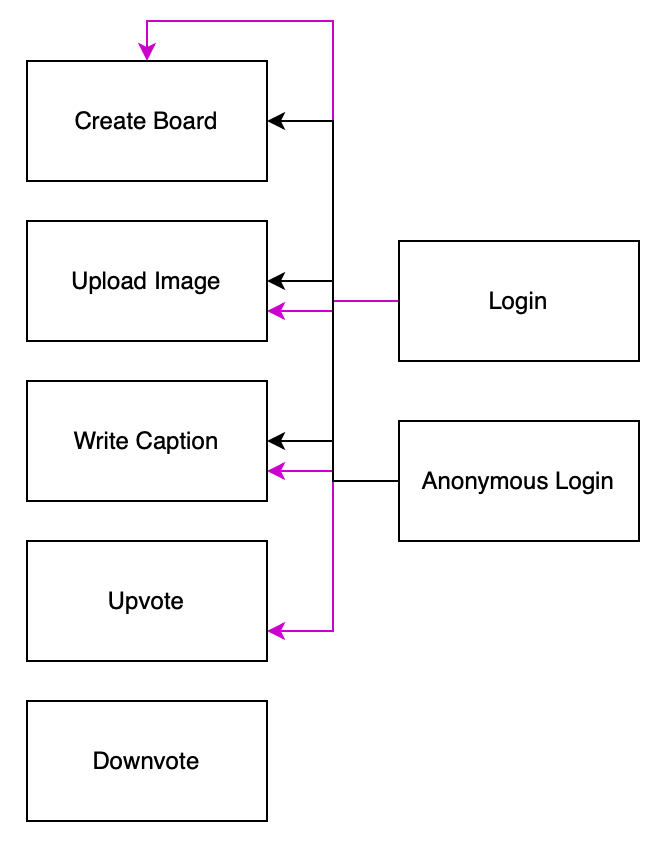
\includegraphics[width=6cm]{system design.png}
\caption{System Design}
\label{fig:sysdesign}
\end{figure}

\section{Functional decomposition tree}
The main functions of the system is decomposed into smaller sub functions or sub-modules and further. The System shall take place following structure of organization after implementation. The decomposition is stable and functions should be made highly cohesive. (fig:\ref{fig:tree})
\begin{figure}[H]
\centering
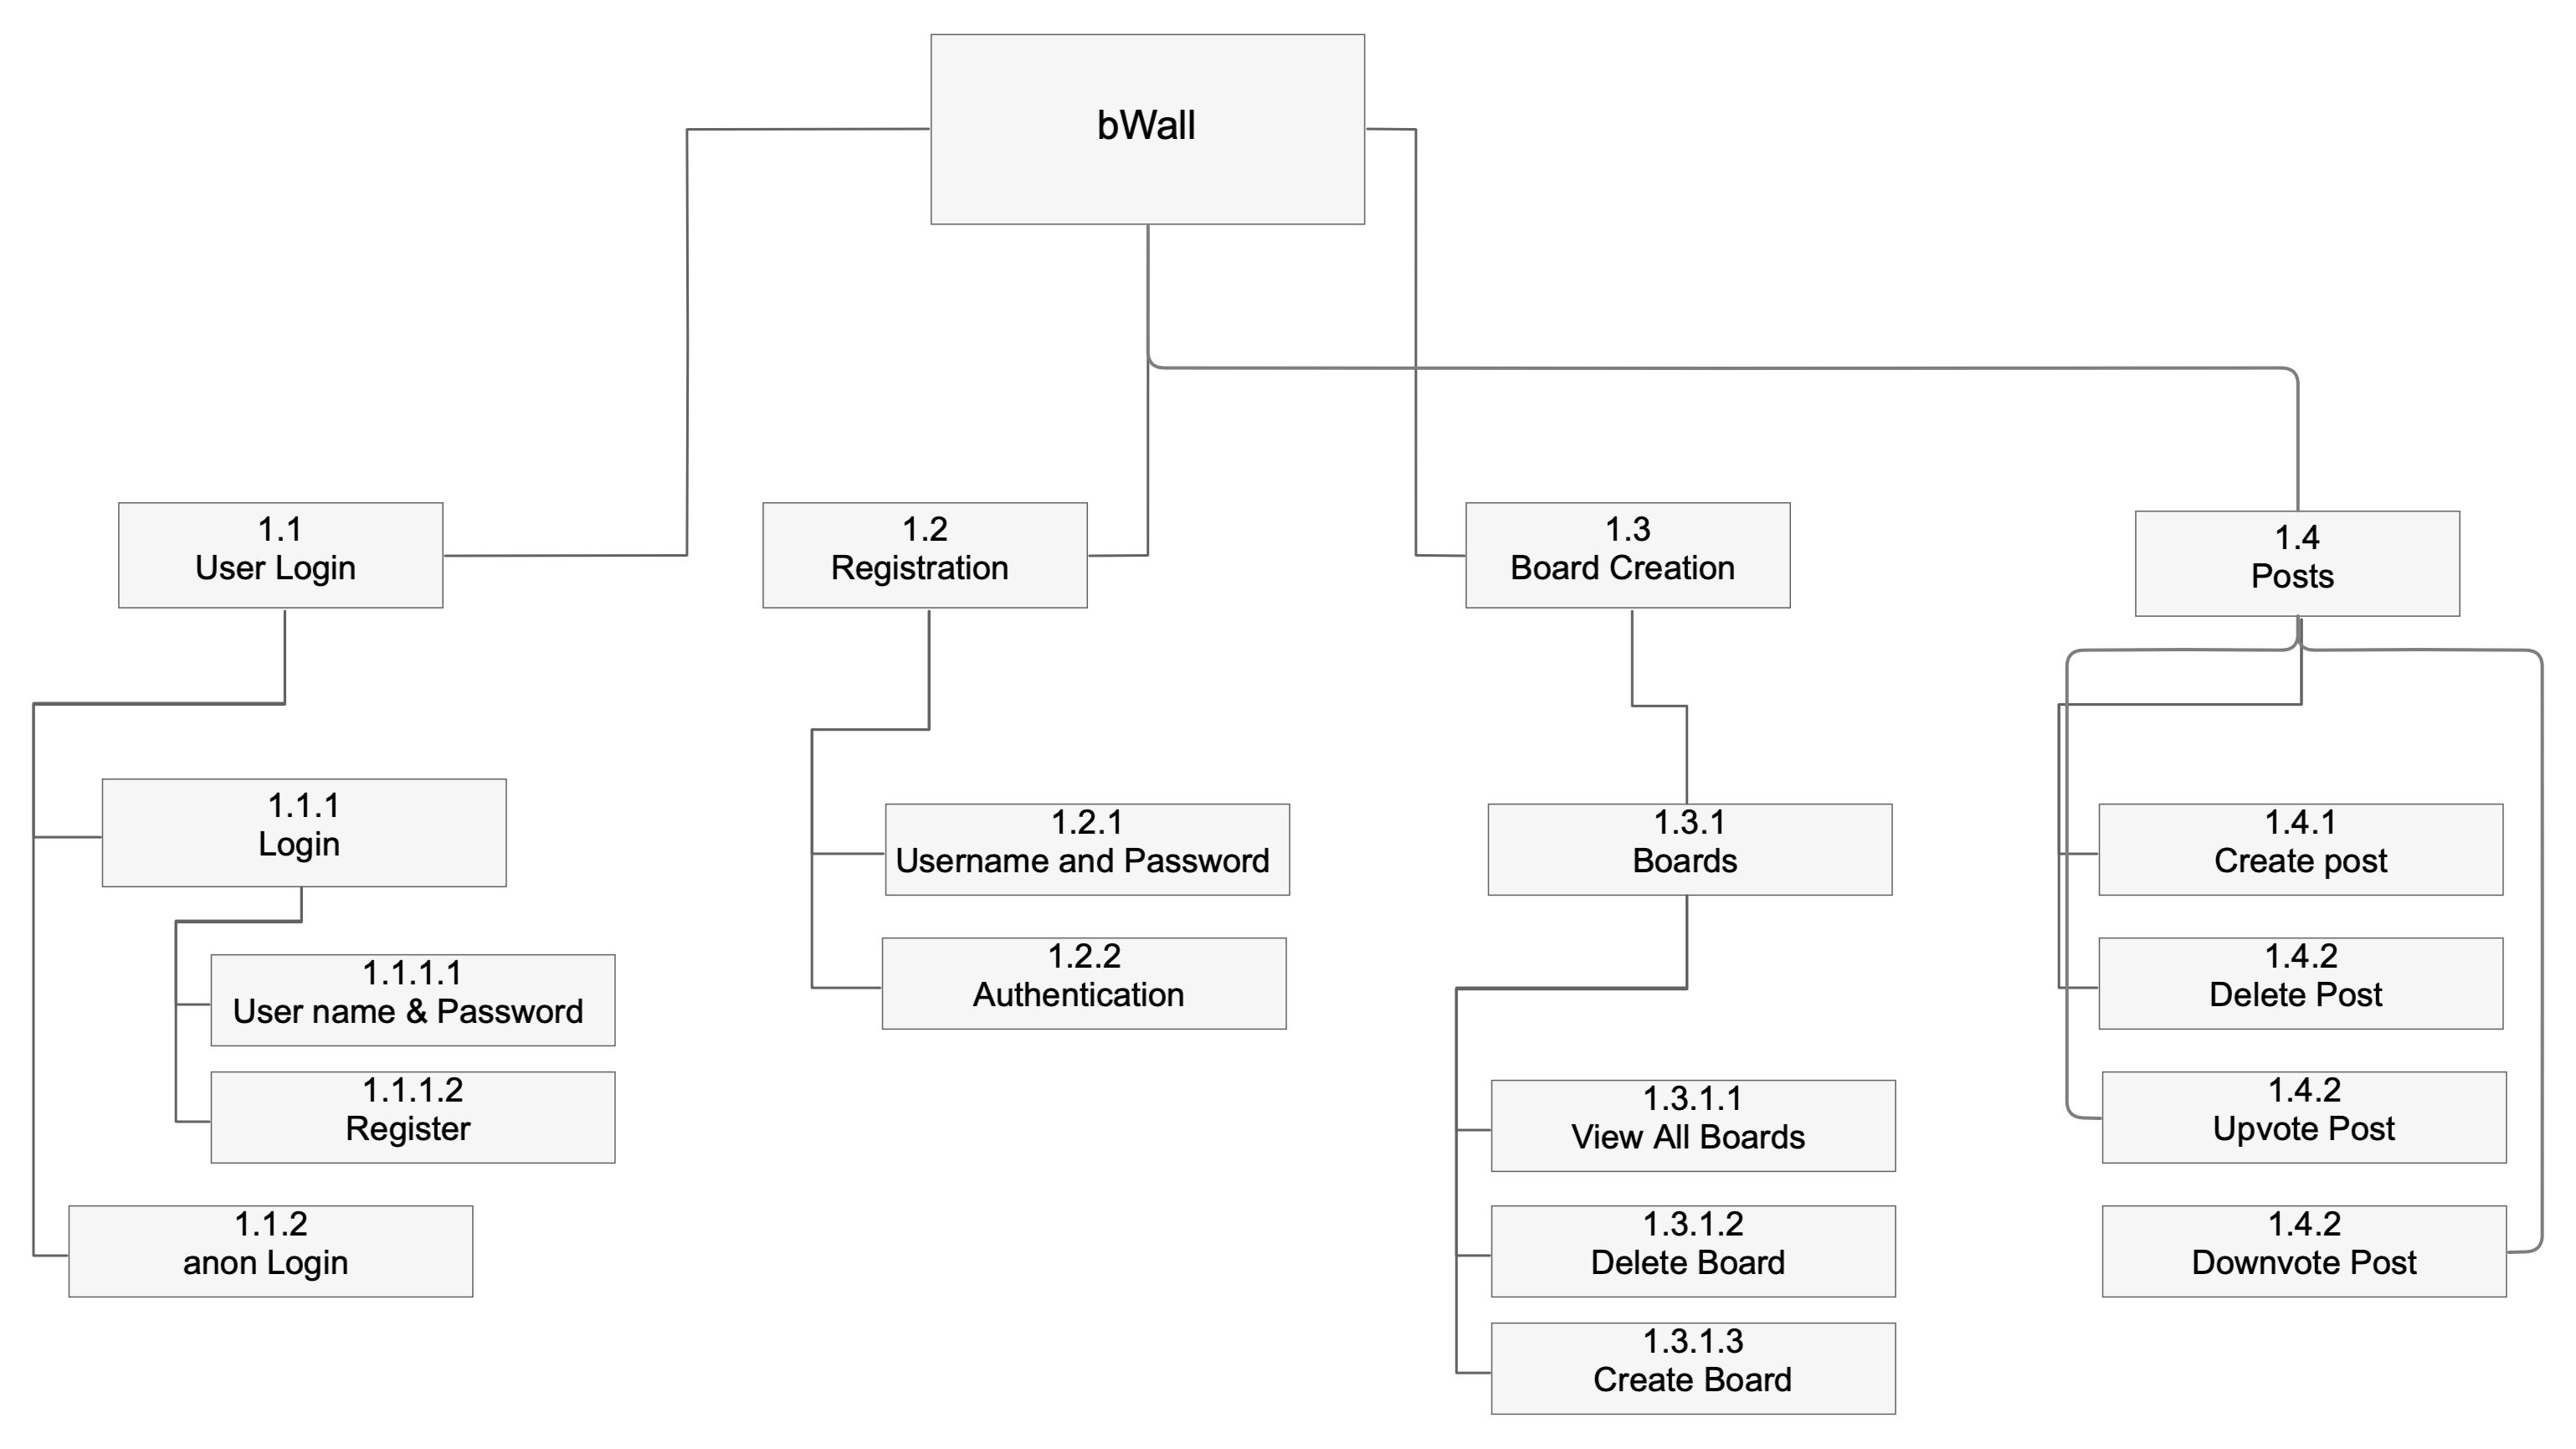
\includegraphics[width=15cm]{Tree.png}
\caption{Functional decomposition tree}
\label{fig:tree}
\end{figure}

Modules involved in the diagram are discussed below:
\begin{itemize}
    \item User Login - This module handles how the user logs in into the system
    \begin{itemize}
        \item Login - Login module for registered users
        \begin{itemize}
            \item Username and password - Enter the username and Password to login into the site
            \item Register - If not registered then register on the website
        \end{itemize}
        \item Anonymous Login - Login anonymously without registering
    \end{itemize}
    \item Registration - This module helps user to register on the website
    \begin{itemize}
        \item Username and password - Enter the username and Password required login into the site
        \item Authentication - the username is authenticated uasing email address
    \end{itemize}
    \item Boards
    \begin{itemize}
        \item View Board - view all the boards created
        \item Add Board - Create a new board
        item Delete Board - Delete a particular Board
    \end{itemize}
    \item Posts
    \begin{itemize}
        \item Create Post - Create a new Post
        \item Delete Post - Delete an existing post on the website
        \item Upvote - Upvote a post user likes
        \item Downvote - Downvote a post user dislikes
    \end{itemize}
\end{itemize}

\section{Context Diagram}
\begin{figure}[H]
\centering
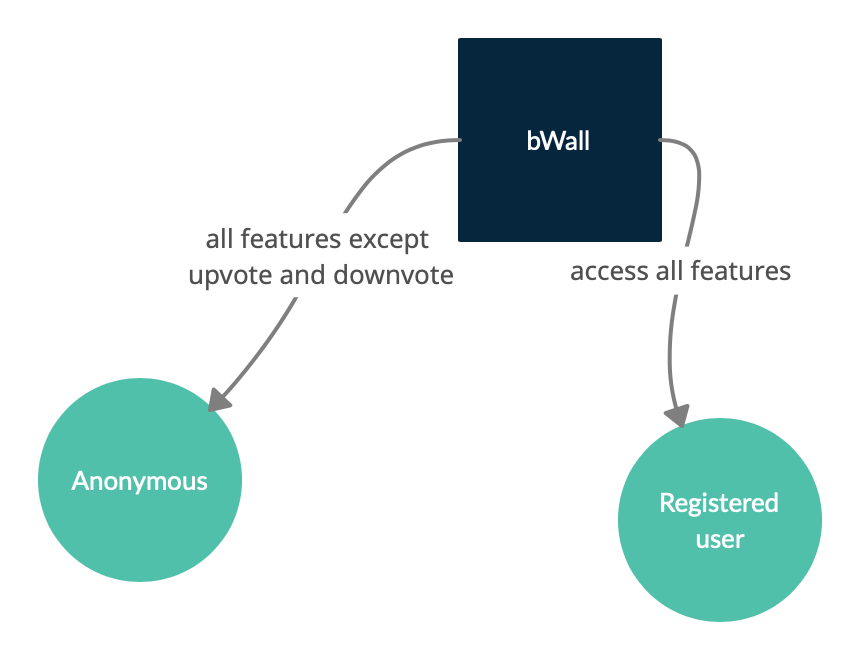
\includegraphics[width=9cm]{dfd0-2.png}
\caption{Context Interaction Diagram}
\label{fig:context}
\end{figure}

\section{Data Dictionary}

\begin{tabularx}{\textwidth} { 
  | >{\raggedright\arraybackslash}X 
  | >{\raggedright\arraybackslash}X
  | >{\raggedright\arraybackslash}X
  | >{\raggedright\arraybackslash}X |}
 \hline
  & \textbf{Field} & \textbf{Type} & \textbf{Property} \\
 \hline
 \textbf{User} & ID & Integer & Primary Key, NOT NULL \\
 \hline
 & username & varchar(150) & NOT NULL\\
 \hline
 & password & varchar(50) & NOT NULL \\
 \hline
 & joinedon & datetime & NOT NULL \\
 \hline
 & isactive & bool & NOT NULL \\
 \hline
 & & & \\
 \hline
 \textbf{Posts} & postid & integer & PRIMARY KEY\\
 \hline
 & image file & text & \\
 \hline
 & username & varchar(150) & \\
 \hline
 & datecreated & datetime & NOT NULL \\
 \hline
 & board & text & \\
 \hline
 & & &\\
 \textbf{Boards} & boardid & integer & PRIMARY KEY\\
 \hline
  & boardshortname & text & NOT NULL\\
 \hline
  & boarddescription & text & NOT NULL\\
 \hline
 & & &\\
 \hline
 \textbf{Reply} & replyid & integer & PRIMARY KEY\\
 \hline
 & board & text & NOT NULL\\
 \hline
 & replyimage & text & NOT NULL\\
 \hline
 & username & text & NOT NULL\\
 \hline
 & date & datetime & NOT NULL\\
 \hline
 & posttext & text & NOT NULL\\
 \hline
\end{tabularx}

\chapter{Software Interface Design}

\section{Principles}

\begin{itemize}
    \item The Concept of Structural - UI is organized in such a way that related things are combined together and unrelated things are separated.
    \item The Concept of Simplicity - It is easy to follow the provided interface. In the case of a mistake, the system displays an error message.
    \item The Concept of Visibility - All system’s functions are available through UI. It does not overwhelm users with too many alternatives.
    \item The Concept of Feedback - Through the system of messages, the design keeps users informed of actions, errors, or exceptions.
    \item The Concept of Reusability - In design, the same names were used to perform the same operations with different objects in order to reduce ambiguity.
\end{itemize}

\section{UI Components\index{user interface}}
This section covers the details of the required user interfaces 

\begin{figure}[H]
\centering
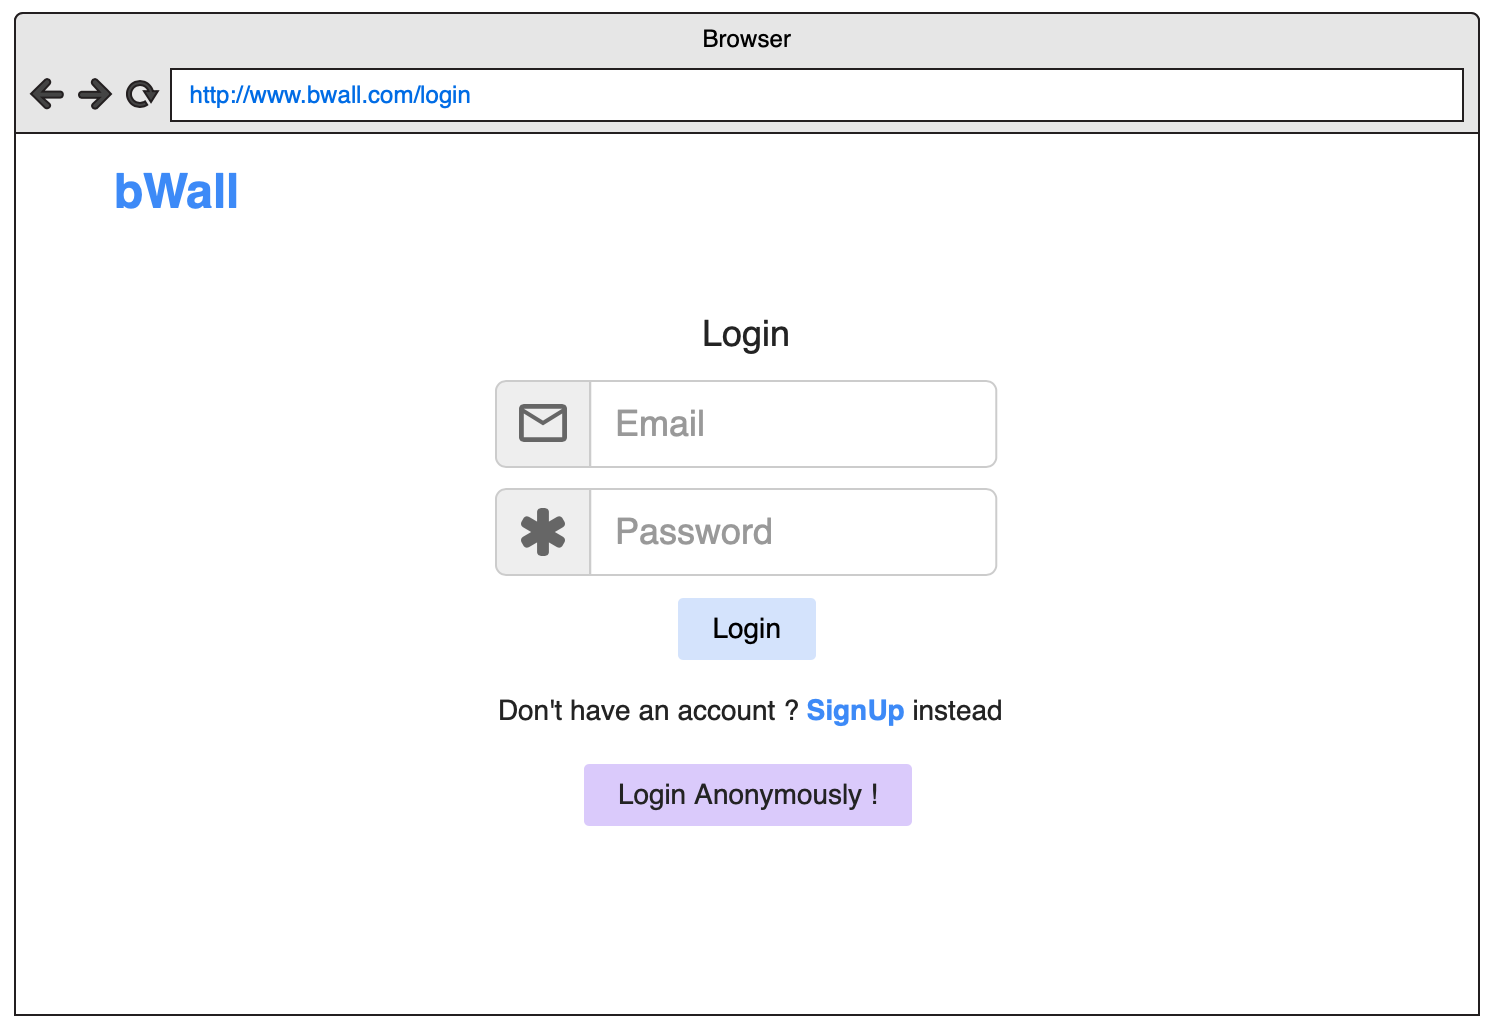
\includegraphics[width=12cm]{uilogin.png}
\caption{Login UI\index{login UI}}
\label{fig:loginui}
\end{figure}
This is the first component that the user will see when he/she will open the site. In the login UI (fig:\ref{fig:loginui}) user will be provided with two input fields of type email and password. User need to provide both and click on login button. If a user is new to the website they can also click on signup to register themselves or they can choose to browse anonymously.

Similarly the signup page (fig:\ref{fig:signupui}) contains two input fields of type email and password. After entering the details user can signup and the account will be created.

View Interface (fig:\ref{fig:viewinterfaceui}) holds all the details of current posts and different types of boards present in the website. This also is the first page after login and hold various options such as view profile, create board, etc.

\begin{figure}[H]
\centering
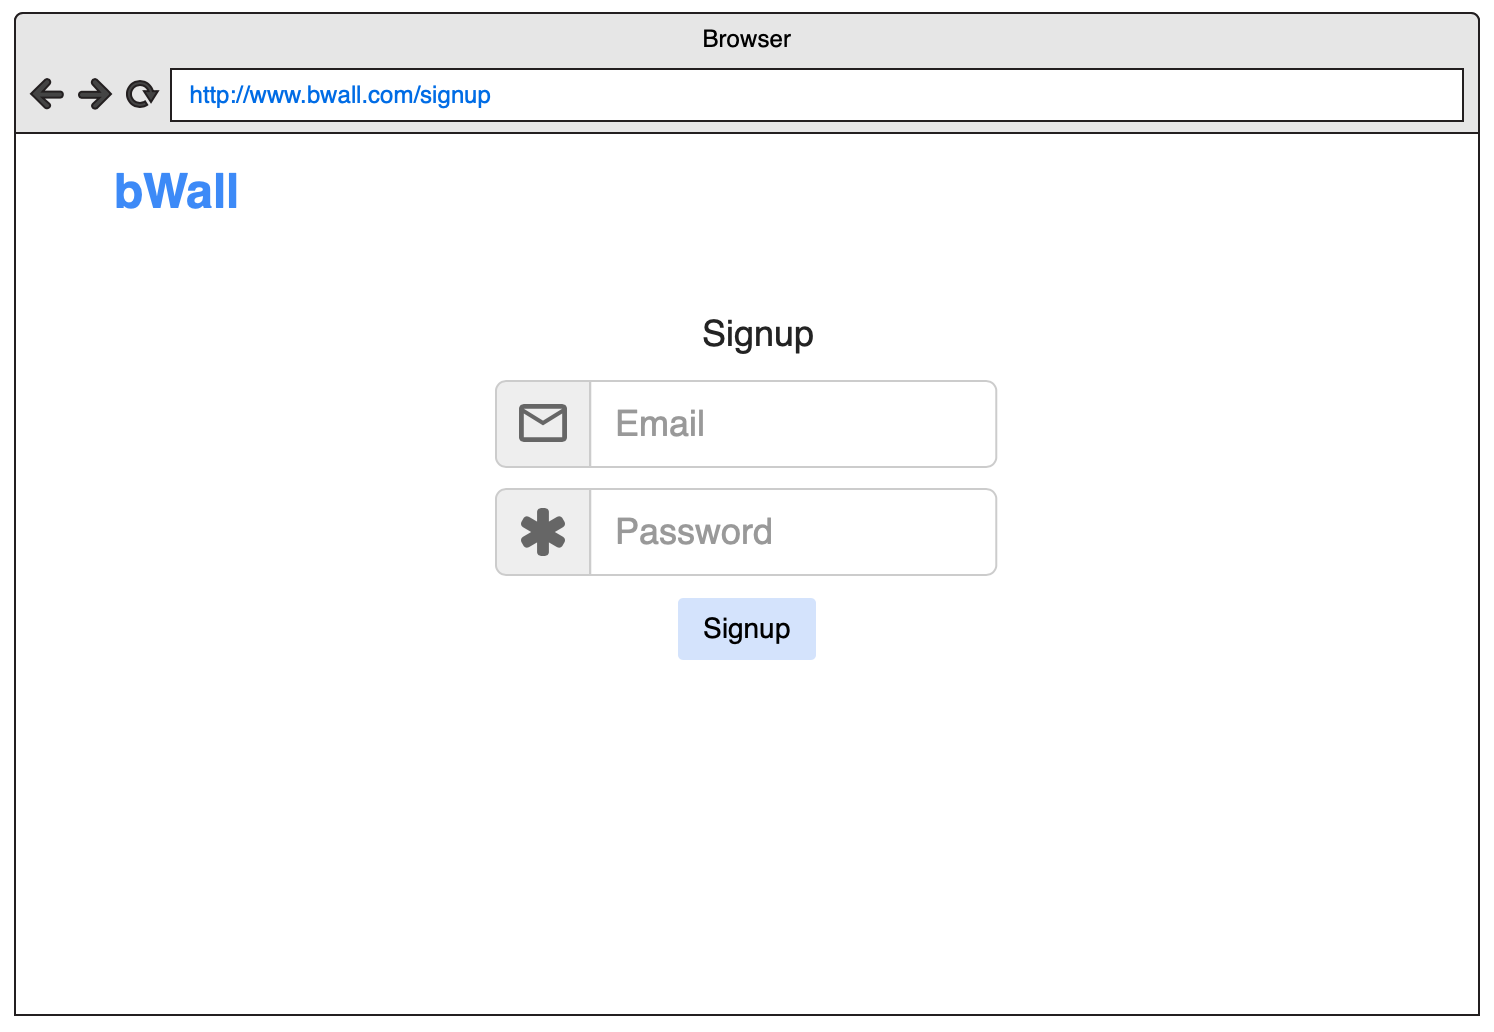
\includegraphics[width=12cm]{uisignup.png}
\caption{SignUp UI\index{signup UI}}
\label{fig:signupui}
\end{figure}
\begin{figure}[H]
\centering
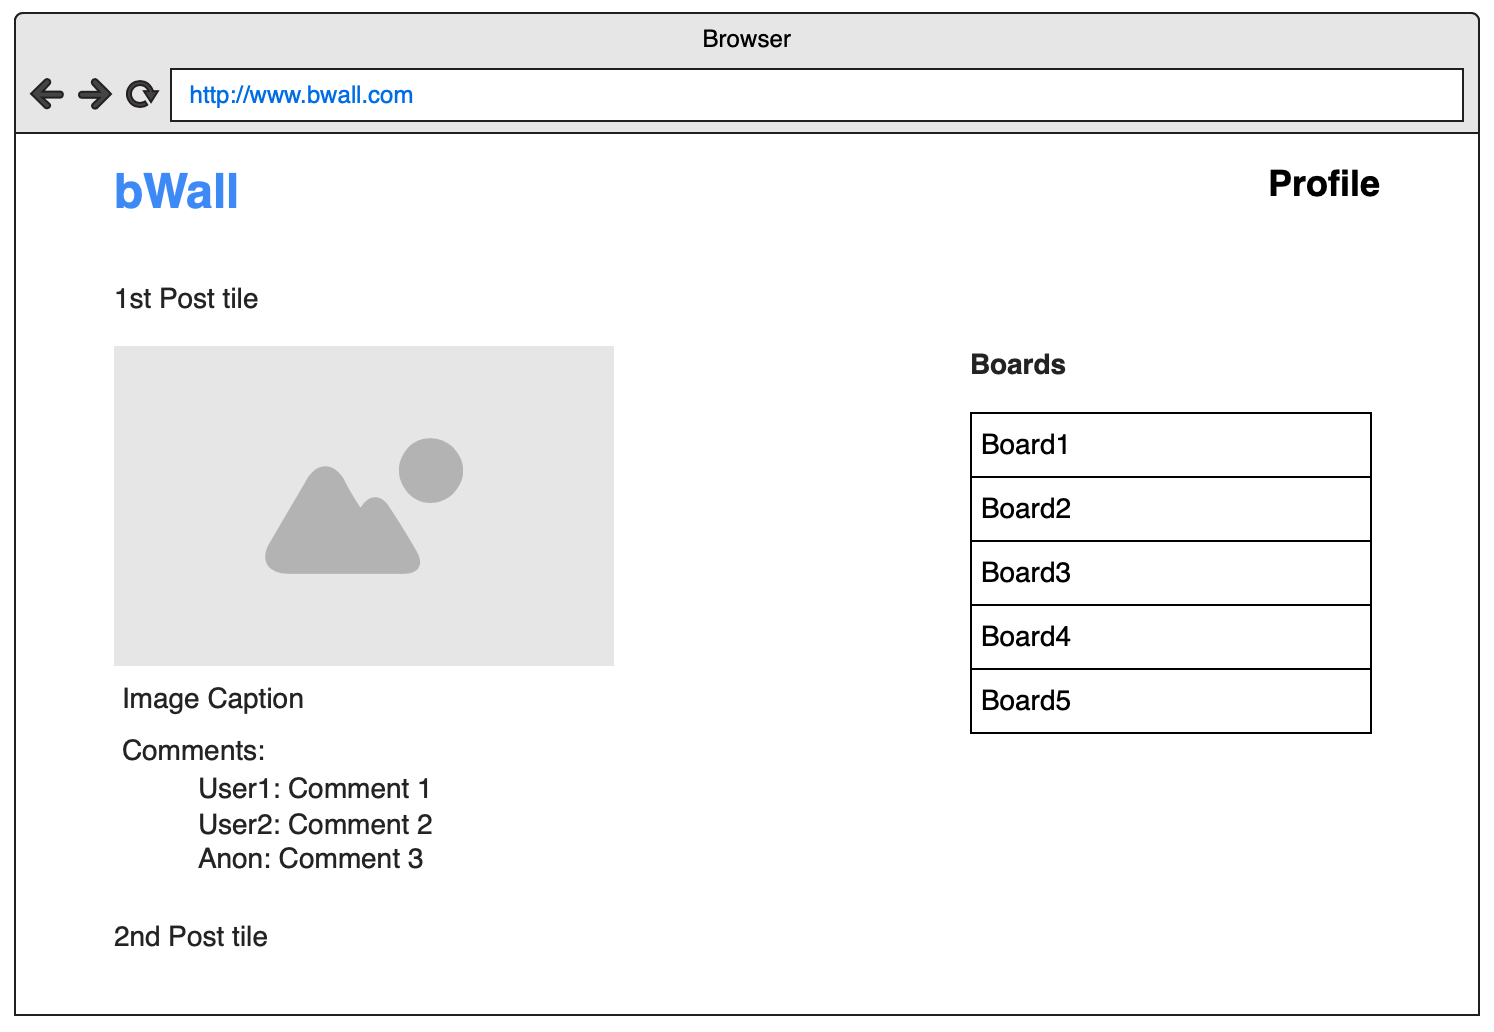
\includegraphics[width=12cm]{uiviewinterface.png}
\caption{View Interface\index{view interface UI}}
\label{fig:viewinterfaceui}
\end{figure}
\begin{figure}[H]
\centering
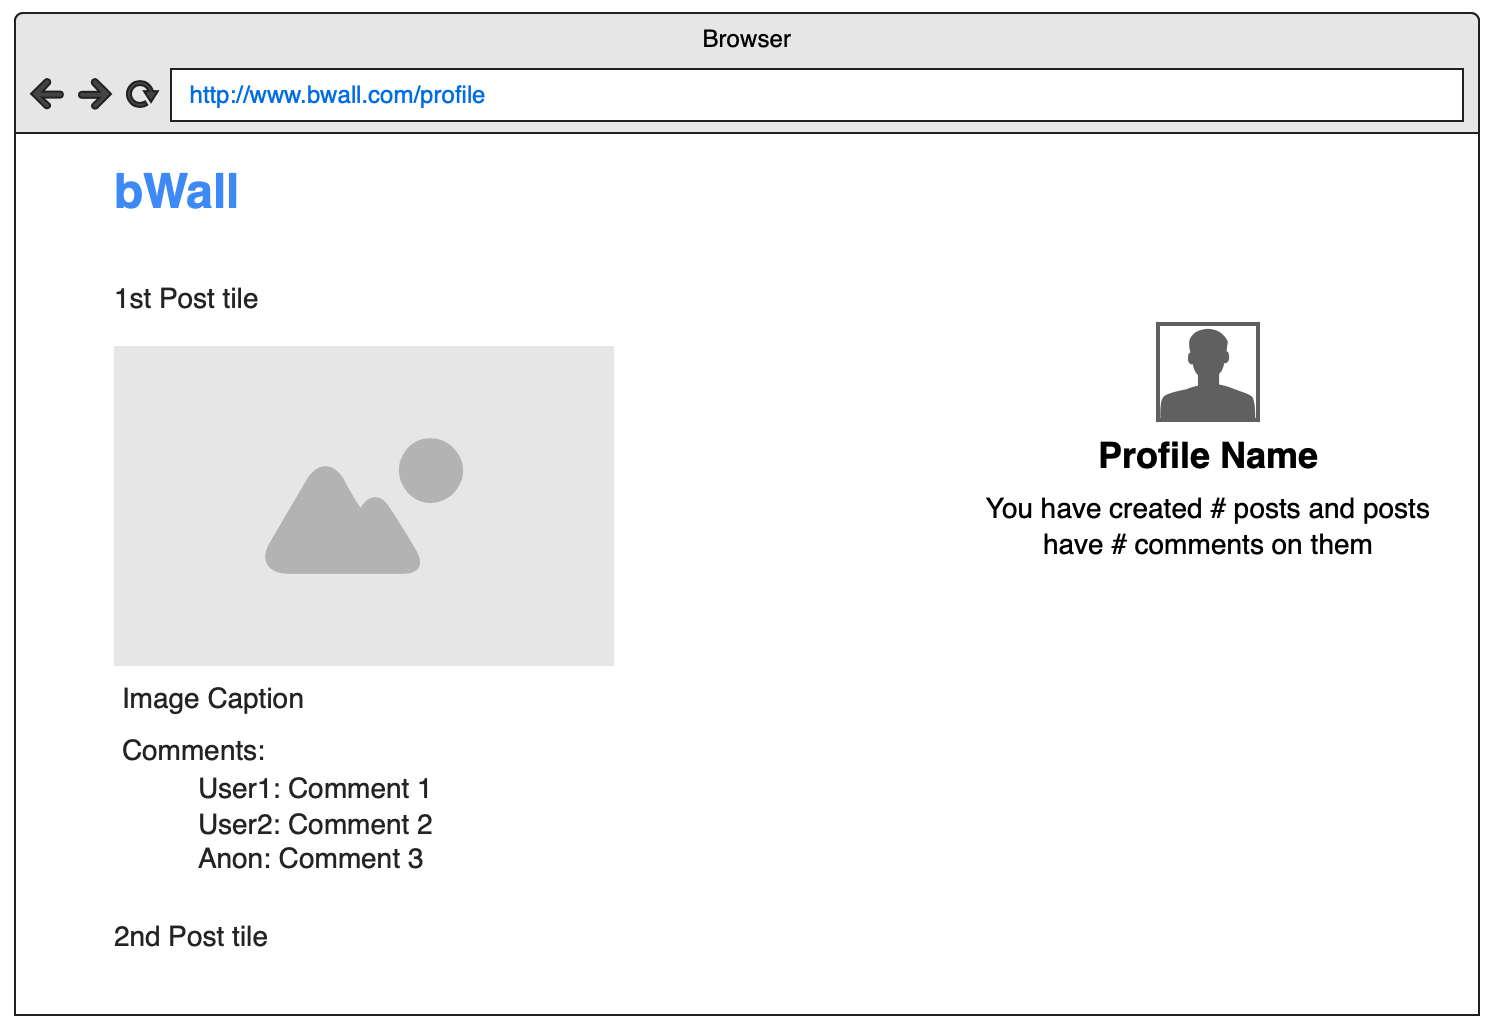
\includegraphics[width=12cm]{uiviewprofile.png}
\caption{Profile UI\index{profile UI}}
\label{fig:profileui}
\end{figure}
\begin{figure}[H]
\centering
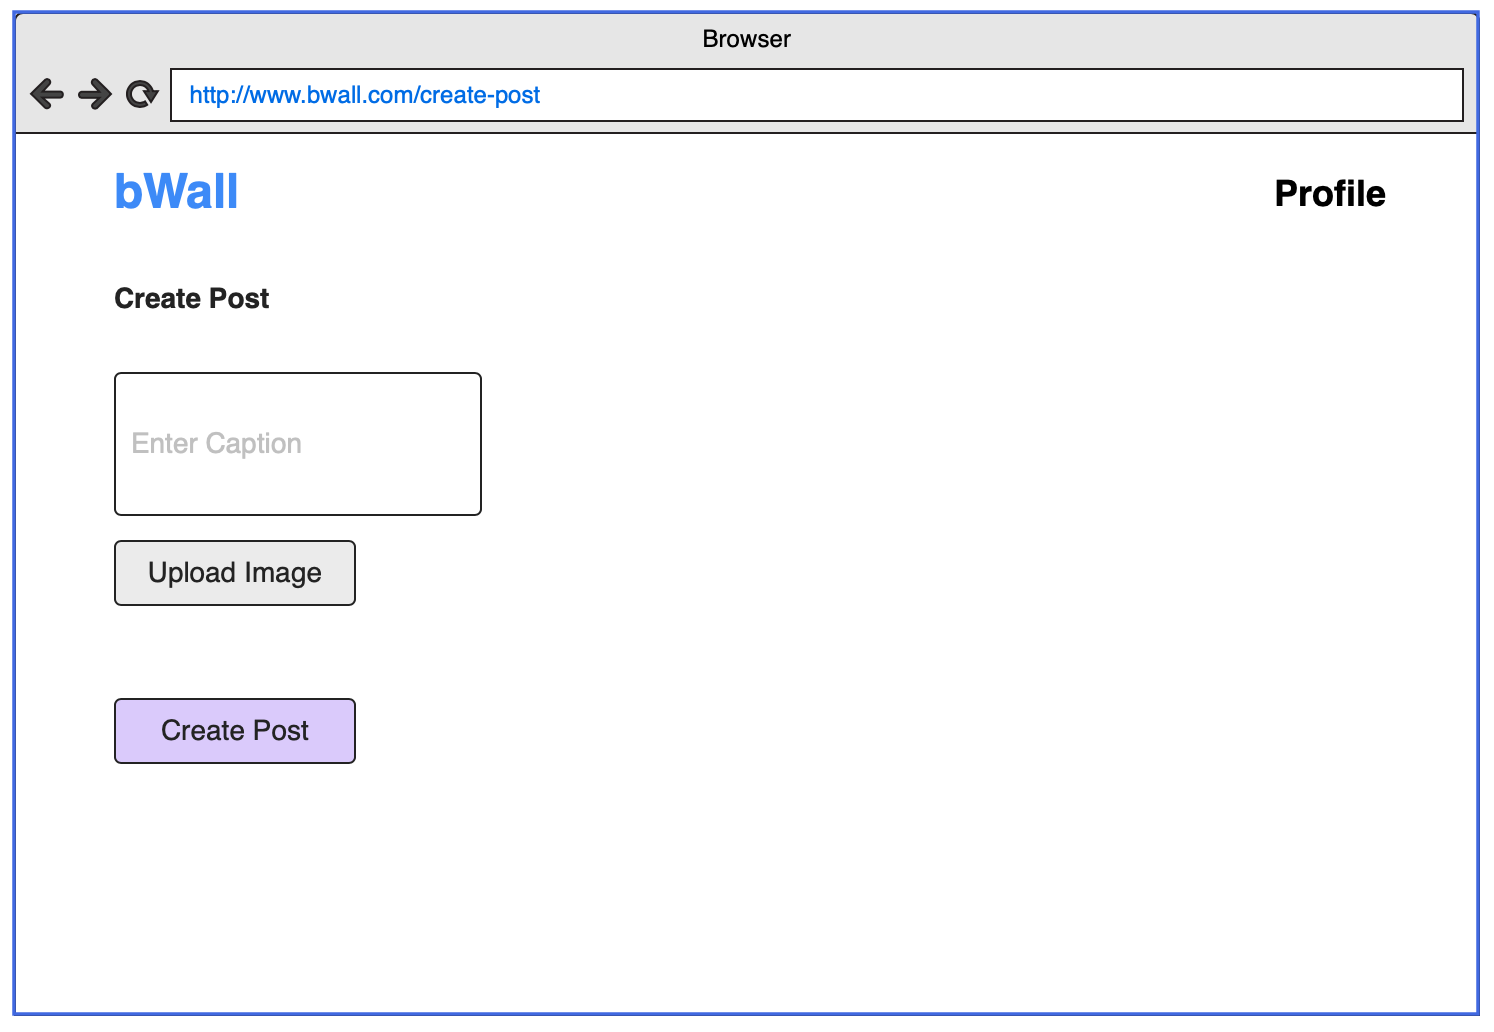
\includegraphics[width=12cm]{uicreatepost.png}
\caption{Create Post UI\index{create post UI}}
\label{fig:createpostui}
\end{figure}

The profile page (fig:\ref{fig:profileui}) contains the posts details created by the specific user. Its also shows the count of number of posts the user has created and the number of comments user as posted.

\begin{figure}[H]
\centering
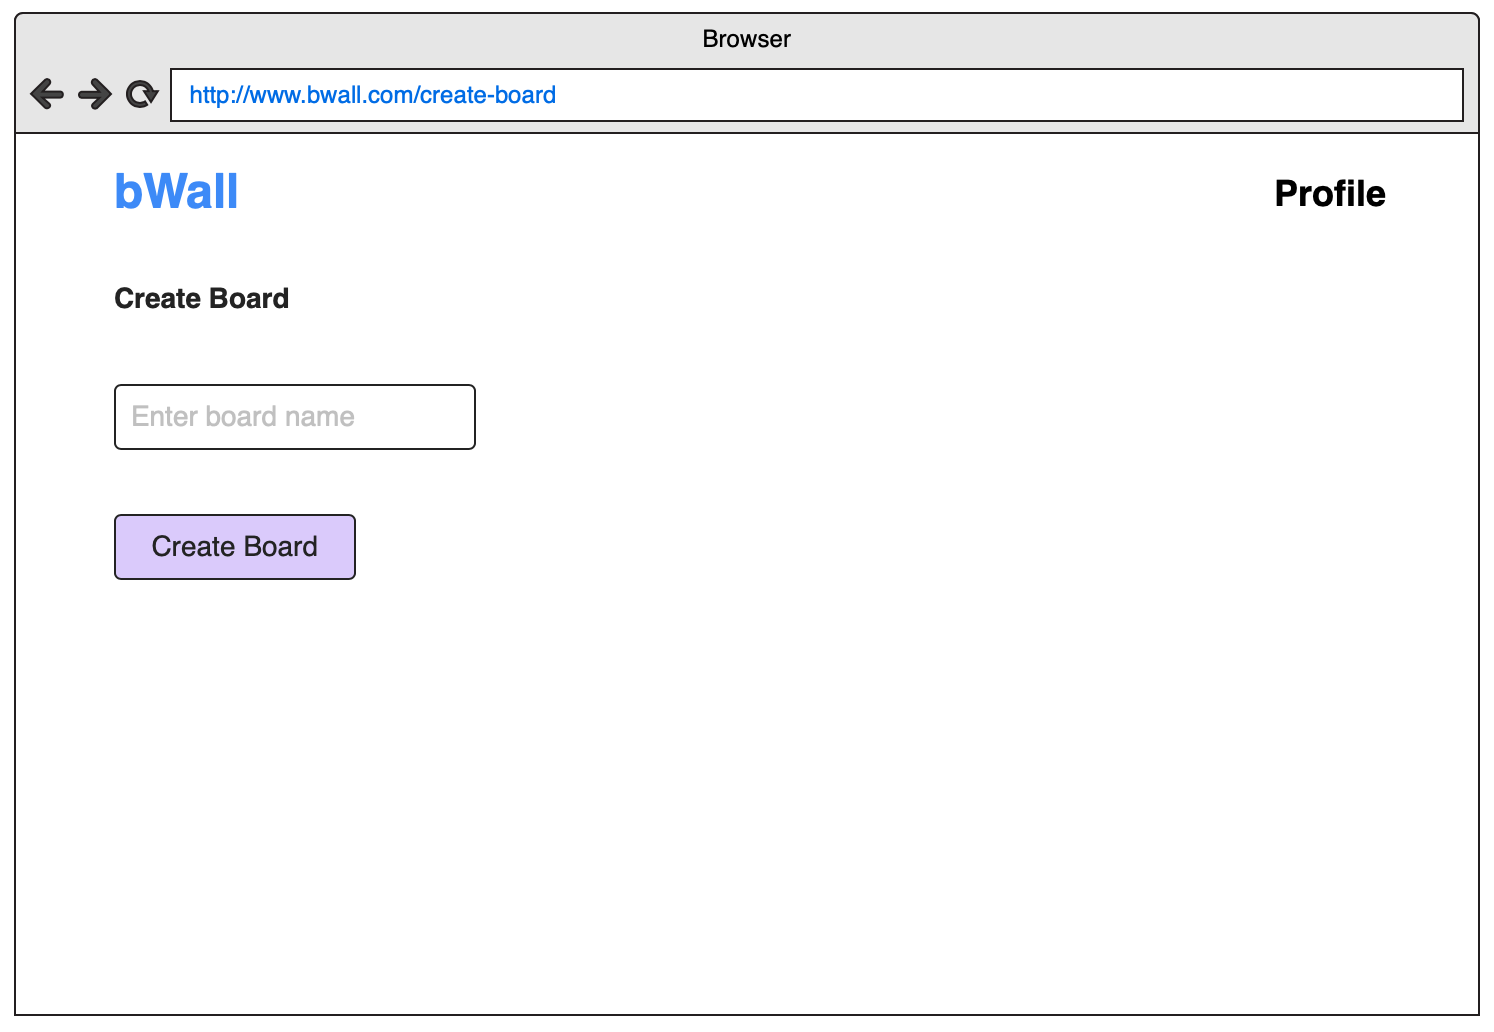
\includegraphics[width=12cm]{uicreateboard.png}
\caption{Create Board UI\index{create board UI}}
\label{fig:createboardui}
\end{figure}

Create post page (fig:\ref{fig:createpostui}) will allow user to create posts. Here user will be provided with the input field to enter the feed text and an option to upload the image.

Create board page (fig:\ref{fig:createboardui}) works in the similar fashion to that of create post page but only difference being that a new board will be created.

There can also be other UI elements to the website but only high-level UI elements are discussed here. There will also be other UI elements such as 404 page, logout page, terms and conditions page, etc.






\end{document}
